\section{\retro\ Design}

% \begin{figure}[!t]
% \vskip -0.03in
%   \centering
%       {
%         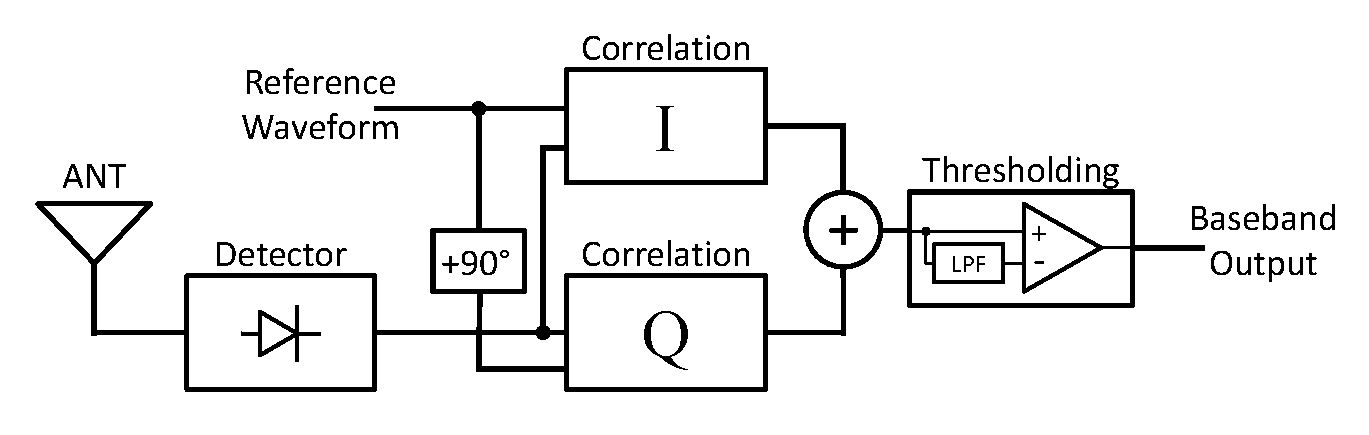
\epsfig{file=../figures/corr-bd.eps, width=0.6\columnwidth}
%       }
% \caption{{\bf System Diagram} (a) \vitag\ and (b) Modified LED.}
% \label{fig:sysdiagram}
% \vskip -0.05in
% \end{figure}

\begin{figure*}[!t]
\vskip -0.1in
\centering
{\footnotesize
\begin{tabular}{cc}
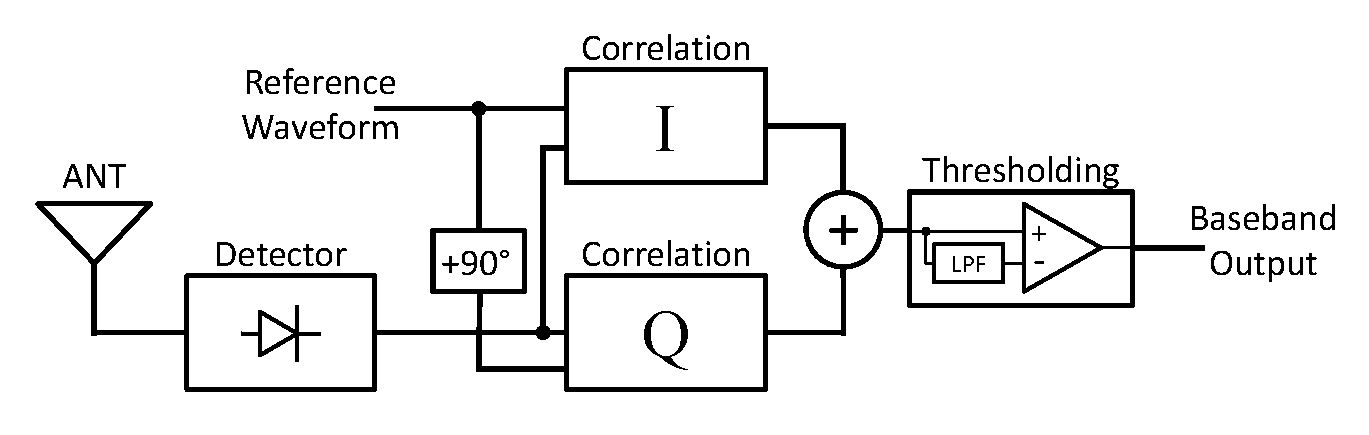
\epsfig{file=../figures/corr-bd.eps, width=\columnwidth} & 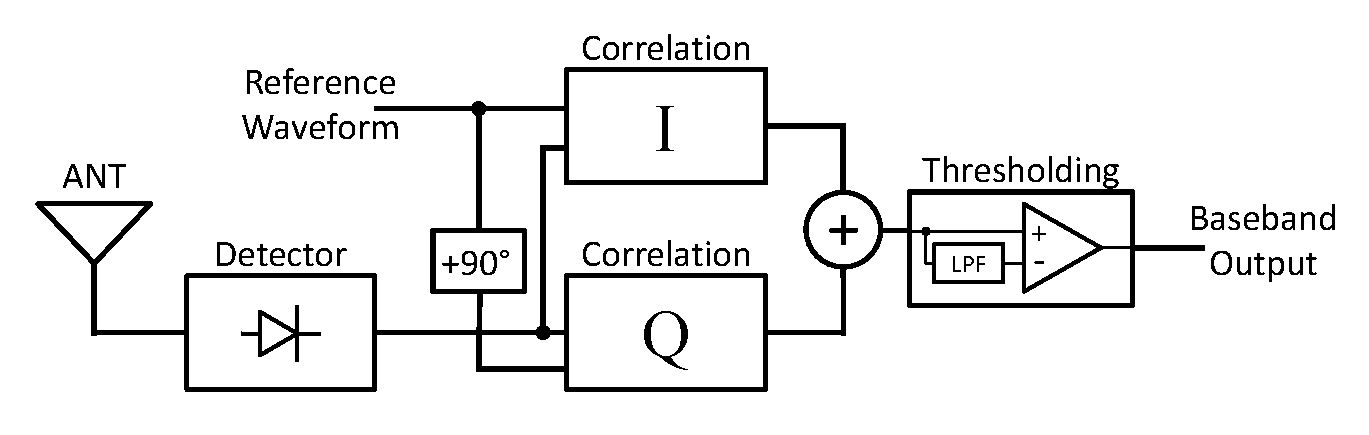
\epsfig{file=../figures/corr-bd.eps, width=\columnwidth}\\
{(a) \vitag\ Block Diagram} & {(b) LED BLock Diagram}\\
\end{tabular}
}
\vskip -0.1in
\caption{\footnotesize{\bf System Diagram.} Blah Blah.}
\label{fig:sysdiagram}
\vspace{-1em}
\end{figure*}

\retro\ is a new form of communication in which battery-free \vitag\/s can communicate with LEDs without any additional infrastructure. Harvesting LED light energy, a \vitag\ reflects visible light signals to communicate. Because of the ubiquitous deployment of illuminating LEDs, building such a system will enable ubiquitous communications at an unprecedented scale. It will also enhance the security of current RFID systems as it limits the uplink signal exposure to line-of-sight, and the use of retro-reflectors will further focus the signal to an even thiner area, leaving less chance for the hidden attackers and sniffers to temper the system.

Designing such a system, however, faces several challenges, which we will break down in the following subsections, and we describe how our design address these challenges.


%Designing such tags, however, is challenging for four reasons: First, the visible light that carries data is interleaving with intensive interference, such as radios operating at the same frequency, and the light emitted from the LEDs that also carries data and its reflections from surrounding walls, thus making an interference-intensive receiving condition for both \vitag\ and \reader. Second, the signal is exposed to noise, such as the existing environmental lights that is subject to constant changing, human-body-movement-caused noise, and the noise caused by the hardware system itself. Third, to emit modulated light from \vitag\ and make it detectable by \reader\ on a battery-free tag is challenging in that modulating signals on visible light bands is power-consuming with respect to the goal of being battery-free. Finally, to integrate the system to off-the-shelf LED lights while keeping the brightness of the lights constant is challenging. In the rest of this section and the next section, we describe how our design addresses the above challenges.




\subsection{Overview}
Fig.~\ref{fig:sysdiagram} (a) shows a block diagram of our \vitag\ design. It consists of a transmitter, a receiver, an MCU and a harvester. The transmitter and receiver communicate by modulated backscattering of visible light signals, and the harvester absorbs energy from visible lights to power the device. Further, they operate independently of each other. The receiver immediately awakes the MCU by rising the tag voltage to a certain value and enabling the analog circuit to start receiving as it detects a data packet coming in. The MCU then shuts down the analog circuit and powers up the transmitting circuit. The receiving circuit and the transmitting circuit work alternately to save energy. Alongside the communication modules is the energy harvester, which consists of a number of solar cells that transfer visible light energy into electric energy. The harvester sets the upper bound of the power \vitag\ can take on, thus posing a strict constraint to the design of each component on the tag.

Fig.~\ref{fig:sysdiagram} (b) shows a block diagram of our \reader\ design. The major part of it is an LED bulb that emits fast-fluctuating light human eyes cannot detect flickering in. \reader\ builds on off-the-shelf LEDs and makes minor modifications on them. It consists of a transmitter, a receiver and an MCU. The transmitter encodes and modulates the data, feeding the data to the LED for transmission, while keeping the LED not flickering and with dimming support. The transmitter also takes the goal of making \vitag\ battery-free in mind, emitting lights with data such that \vitag\ can demodulate and decode the data at a low energy cost. The receiver deals with the light backscattered from \vitag, and also cancels noise and interference as much as possible. The MCU processes the data transmitted from \vitag.

Next, we describe our design of the transmitter and receiver on the \vitag\ and LED in more detail.





\subsection{\reader\ Transmitter}

As shown in Fig.~\ref{fig:sysdiagram} (b), the transmitter on \reader\ is composed of a crystal oscillator that runs at 1MHz, and an MCU followed by two amplifiers. The data generated by the MCU controls a switch on waves generated by the crystal oscillator so that the data is modulated. The modulated signal will then be amplified and fed to a LED. To make sure the brightness of the LED does not pose a difference between the transmitting and not transmitting state, we add a DC component of a particular value to signal when at the transmitting state such that the the average strength of the light at the transmitting state is the same as solely lighting. The magnitude of the DC component is such that it is adjustable to provide dimming support as what existing LEDs are capable of. In addition to the dimming support, flickers are avoided in \reader\ transmitter. We use 10kHz as the data rate, which far exceeds the frequency (200 Hz) below which human eyes will feel of fluctuations, which could disturbing and unacceptable. 

We note the following about our design: Firstly, we use a white-colored LED, which emits electromagnetic waves of wavelengths between 380 and 780 nm. The highest flickering frequency of the LED  with full on/off transitioning is 1MHz, and we are exploiting the flickering rate to its fullest, in order to leave room for downlink data rate as high as possible. 

Secondly, different components in the transmitter on the reader side require different voltage supply. We are using two DC/DCs to boost the voltage for the switch and the amplifiers. Specifically, the voltage used for supply the crystal oscillator, the amplifiers for the MCU-output signals and the switch is 5V, and the voltage for the amplifiers for the RF signals is 12V. 

Finally, the 1MHz frequency, as mentioned earlier, is used because of the full flickering capability we would like to draw from the LED. However, around this frequency with a bandwidth on the order of 100kHz, there are  commercial radios using AM modulation. For example, there are radios from 540 through 1610 kHz with 10 kHz spacing in America. Another form is situated at a similar spectrum spanning from 531 to 1611 kHz with 9 kHz spacing. These are sources of interference to what we transmit with the LED, and we are going to address this issue with the receiver design on the reader, which also deals with other sources of interference and noise.





\subsection{\vitag\ Receiver}
Looking along the flow of the signal, we then describe the design of our \vitag\ receiver. Designing a visible light receiver entails a light sensor that captures the fluctuation of the visible light with a satisfying bandwidth. Then the captured signals go through filters, detectors/demodulators, and another feedback amplifier before sending to a comparator be digitized. On top of these, the design should be energy-efficient, such that the harvested energy is enough to supply the operation of the tag. We avoid using power-demanding ADCs while achieving \hl{data rate} at \hl{x} accuracy at the distance of \hl{sss} using only analog elements and a low-power MCU. The block diagram of the receiver is presented in Fig.~\ref{fig:sysdiagram} (a).

\subsubsection{Extracting Information from the Visible Light}
\reader\ transmitted signals will first be sensed by a light sensor BPW34. Since the light sensor has an equivalent capacitance, along with an inductor parallel to it, it performs preliminary front-end filtering. Since natural lights do not have a component at 1MHz, this filter does a good job singling out the useful signal and filtering out lights from other sources. Next, two amplifiers will successively increase the RF signal strength while avoiding auto-excitation using feedback mechanisms. After the preliminary filtering and amplification, the signal is ready for demodulation. These processing blocks consume power up to \hl{aaa}, of which the light sensor consumes \hl{ddd}, and they are shut down once the tag turns into the transmitting mode in order to save energy.

Next, we describe the mechanism of our simple yet powerful signal detector under a strict energy constraint. The circuit is a variant of an envelope detector. Unlike a conventional envelope detector, the detector is targeted specifically for energy-constraint conditions, while providing a higher gain and a bigger bandwidth. So it is especially suitable for \vitag, where the downlink data rate is high but with being battery-free as its goal. At a high level, it contains a constant current source, a diode, and a frequency selection amplifier. The constant current source sets the current that flows into the base of the triode in the frequency selection amplifier, making it work in the near-conduction state, such that when the positive half of the signal that has an average of 0 flows in, the amplifier is turned on and the signal is amplified. In contrast, when the negative half of the signal flows in, the amplifier is turned off, such that looking at the wave that comes out of the amplifier, the high frequency component, the carrier wave, is cut off half. Then the signal passes through an RC filter, which further smooths the signal. This smoothen signal has little carrier wave component in it, ready to be fed to a comparator for digitization. Overall, the bandwidth of this envelope detector is \hl{sss}, the power that supplies it is \hl{aa}, and the gain it multiplies to the input signal is \hl{sss}, as compared to \hl{aa, bb, cc}, respectively, when using a normal envelope detector. Considering our energy budget on \vitag, this amount of saving is significant. 

We illustrate the signal at the input port, at the output port of a traditional envelope detector and at the output port of our low-power envelope detector in Fig.~\ref{fig:sysdiagram} (a). It shows that compared to the output of a traditional detector, the output of our detector is smoother, while having a higher gain. We will see in the following section that the smoother version of the signal is easier to detect using our comparison decoder under the Manchester coding assumption.

\subsubsection{Decoding on an Ultra-Low-Power Device}

Challenges:
\begin{Itemize}
\item Demodulating and decoding the high throughput LED-transmitted data is power consuming. 
\item Transmitting with the LCD at a high toggling frequency consumes even more power than the receiver.
\end{Itemize}

Solution principles:
\begin{Itemize}
\item Use analog components as many as possible (to avoid analog-to-digital converters (ADCs)) and avoid complicated digital signal processing on the mobile end. 
\item Recycle energy spared by the LCD at every toggle.
\end{Itemize}

The output of the envelope detector produces a smoothen wave, yet it is still analog, with continuous values. In principle, a receiver with an ADC can distinguish between the two signal levels by processing the digital samples. Specifically, say we have two signal with different voltages, $V_0$ and $V_1$, $V_0 > V_1$, where $V_0$ and $V_1$ correspond to the power levels for the zero and one bits. To distinguish between then, the receiver would first compute a threshold value. If the duty cycle of the signal is $50\%$, and probabilities of the occurrence of zeros and ones are equal, then the threshold is the average of the two power levels. When the received signal is greater than this threshold, we conclude that the received signal is $V_1$; otherwise, we conclude that the received signal is $V_0$.

Since we choose to eliminate the need for a full ADC in order to reduce power, the receiver is supposed to imitate this operation using analog hardware. This design, though, is slightly different from a conventional ADC, in favor of Manchester coding we use (see~\ref{subsubsec:clockoffset}). The Manchester-encoded signal uses edges to denote bits. Specifically, an \hl{up} edge denotes one, and a \hl{down} edge denotes zero. To achieve consent with this pattern, we design a comparator that detects changes of the voltage. First, using a resister and a capacitor, the comparator sets a time constant that features its detection delay that corresponds to the input data rate. The comparator consistently compares the current analog value $V_{now}$ with the signal value at the last bit $V_{previous}$. If $V_{now} > V_{previous}$, the comparator outputs \hl{one}; otherwise, it outputs \hl{zero}, after a time span of the time constant. 

We note that while a traditional design only performs absolute comparison, our design traces the relative changes in the voltage. Further, using a traditional detector would lead to jagged waveform, which would further cause false comparison results at any edge-oriented comparator. Instead, our comparator design is more suitable for Manchester coding, which is widely adopted for preventing long consecutive ones or zeros in a bit stream, in avoidance of picking a threshold value that is subject to drifting. 





\subsection{\vitag\ Transmitter}
The design of our \vitag\ transmitter builds on off-the-shelf Liquid-Crystal Displays (LCD) and retro-reflectors. The LCD and the retro-reflector combined serve as the modulator for the signal generated by an MCU and amplified on the tag. The LCD's energy is spared each modulation cycle is partially recollected by an energy reuse module that saves $50\%$ of the energy that the tag would have wasted otherwise. The amount of energy saved is of significant importance as to lessening the area of the tag. In addition, the LCD requires a voltage high enough to drive it to its fullest capacity, and this high voltage cannot be directly fed by the low voltage the solar cell can provide. We design a voltage boost module that achieves this with low energy consumption. Overall, the design of the \vitag\ transmitter is presented in Fig.~\ref{fig:sysdiagram} (a).

\subsubsection{LCD and Retro-Reflector-based Modulation}
In the \vitag\ design, we use a retro-reflector to backscatter the incoming light and an LCD put on top of the retro-reflector to modulate the light. In our design, we use a \hl{sss $\times$ bbb} retro-reflector. The reflectivity of the retro-reflector is \hl{sss}, and the Field of View (FoV) is \hl{sss}, which effectively signifies to what degree the reflected signal is focused. The LCD we use is sized \hl{aaa}. 

As electromagnetic waves hit the LCD, the LCD lets the light pass through or blocks it depending on the polarization, i.e., the orientation of the liquid-crystal molecules, in the LCD, which is controlled by the voltage added on it. If the applied voltage is large enough, the liquid crystal molecules are almost completely untwisted and the polarization of the incident light is not rotated as it passes through the liquid crystal layer. This light will then be mainly polarized perpendicular to the second filter, and thus be blocked and the pixel will appear black. The highest voltage applied to the LCD that turns it completely black is \hl{6.1V}, and the lowest voltage with which it starts to be polarized is \hl{2.1V}. We are able to flicker it as fast as \hl{500Hz}. We use the fastest rate as the communication data rate on the uplink, making a \hl{www} power consumption of the LCD. Note, that there are other voltage-controlled reflective materials existing that may have higher flicking rate or lower power. Applying one of those in the system might enhance the energy efficiency and the capacity of the system.  

\subsubsection{Energy Reuse}
The LCD has an equivalent capacitance that corresponds to its periodical charging and discharging. In the discharging phase, if the transmitter has a path along which the current can go all the way from the LCD to the ground, then the energy is wasted. In response, we design an energy reuse module that collects the energy in the LCD discharging phase. The design features a DC/DC converter that boosts the voltage from the lowest voltage that triggers the LCD to the highest. The lowest voltage, as mentioned earlier, is \hl{fff}, which is about the voltage the solar cell array can supply. 

In the charging phase, in which the LCD turns to the blocking mode, the DC/DC boosts the voltage the solar cell supplies to the highest voltage the LCD takes in, as illustrated in Fig.~\ref{fig:sysdiagram} (a). This voltage, through switch $T_0$ the MCU sets to open, applies to the LCD. In this phase, switch $T_1$ is set to close, so the voltage on the LCD gets to pump up until it reaches the discharging phase.

In the discharging phase, the MCU sets the switch $T_0$ to close, and alternatively sets the switch on the discharging path of the LCD $T_1$ to open. Since there is a diode that blocks the only path along which the LCD is supposed to discharge to the ground, the current that flows from the discharging LCD does not go straight to the ground, and instead, it flows back to the DC/DC, charging \hl{$C_0$ and $C_1$}, until the voltage reaches a balance between the LCD and the solar cell. 

The two signals that control the on/off state of the switches are generated by an MCU. When one of the two is set to high, the other is set to low, and vice versa, such that there is only one triode of $T_0$ and $T_1$ open at a time, and so the LCD is either in a charging phase or in a discharging phase, without any conflicts. In addition, we need to make sure that the data rate is slower than the rate at which the two signals from the MCU alternate, so that the voltage on the capacitor-equivalent LCD alternates in a balanced manner in a long run, and $C_0$ and $C_1$ will not constantly be charged or discharged. \vitag\ has \hl{250 bps} data rate, which is smaller than \hl{ccc}, the average time used for charging an empty LCD or discharging a full LCD.






\subsection{\reader\ Receiver}

Challenges:
\begin{Itemize}
\item Detecting the retro-reflected signal against same-band interferences with the LED receiver is hard.
\item The LED must handle clock drifts without explicit synchronization between the LED and the mobile device.   
\end{Itemize}

Solution principles:
\begin{Itemize}
\item Design amplifiers that work at an almost cut-off state to further reduce energy consumption.
\item Design a sliding-window multi-symbol match filter algorithm to remedy clock drifts and LCD-caused signal distortions.
\end{Itemize}

\reader\ captures the signal transmitted by \vitag\ at 250 bps data rate modulated by a 1MHz wave with a light sensor. Upon transferring the fluctuations of the light to voltage, the \reader\ receiver demodulates and decodes the data using RF-end analog circuits and an MCU. While there is less power limit on \reader\ than \vitag, which makes the design more flexible than \vitag, the challenges the \reader\ receiver faces are multi-fold. (1) First, the signal that carries useful information sent by \vitag\ is mixed with the \reader-transmitted signal, which is on a 1MHz carrier as well. What's worse is that since the \reader\ receiver is much closer to the \reader\ transmitter than the \vitag\ transmitter, the strength of the \reader-transmitted signal with the reflections of this signal by the surroundings is in the measurement \hl{ss} times greater than the \vitag-transmitted signal on \reader, making it difficult for the \reader receiver to decouple the two components. (2) Second, the signal carried on 1MHz to be sent by the \reader\ transmitter can also leak to the light sensor, which exacerbates the interference on the light sensor. (3) Third, commercial radios that run on 1MHz could also interfere with the signal that carries useful information. (4) Fourth, the noise caused by the movement of humans and other objects around, along with the circuit noise, could be huge, making the voltage output of the light sensor on \reader\ prone to saturating. In the rest of this section, we describe our \reader\ receiver design (Fig.~\ref{fig:sysdiagram} (b)) that addresses all these challenges, and the techniques that finally make the \vitag\ and \reader\ system practical.

\subsubsection{Extracting Backscatter Information from noise}
Compared with background noise and still-existing interference, the signal strength is weak. For \reader\ receiver, the SINR is \hl{dB}. Specifically, the information bits received \hl{at the light sensor (or after the interference cancellation)} is \hl{dB}, and the interference and noise combined are \hl{dB}. What we finally send to the digital circuit to decode should be a much amplified version of the signal after interference cancellation. Therefore, we need to filter out the carrier wave from the signal and amplify it by \hl{dB}. Using a single amplifier though, is not enough, as there is much more potential of introducing self-excitation to the circuit with too large of an amplification, and the noise introduced by a single amplifier tends to be huge. So we have chosen to apply four separate amplifiers that straddle from the RF-end to the baseband, while performing filtering at each amplifier. The detailed design of this part is the following. To extract the useful information from the noisy background, we first apply an amplifier at the RF end that has the with the amplification of \hl{aa}. This amplifier directly follows the light sensor \hl{or the interference cancellation} with a preliminary LC oscillator that filters out part of the channel noise. Subsequently we add a differential amplifier following a transmission line which decouples the transmitted signal from leaking towards to \reader\ transmitter RF end. The amplification of the differential amplifier is \hl{aa}, with a inductor in parallel with a capacitor that picking out the signal from the carrier wave. Upon filtering, the signal is led to a third amplifier with the amplification of \hl{vv}. The third amplifier is also simultaneously performing filtering, which further picks out a purer signal wave. What follows is the fourth amplifier with feedback and an LC filter. The use of this amplifier is to further increase the signal gain and filter the residual RF-band noise, while bringing the circuit farther from the self-excitation state. After the four levels of amplification, the information signal strength is boosted to \hl{dB}, whereas the background noise is \hl{dB}. And this signal is sent to a envelope detector, which performs regular detection and picks out the baseband signal from that on the 1MHz carrier. 

Overall, this part gives amplification of \hl{dB} on the signal, and achieves \hl{sdd} reduction in the noise. 

\subsubsection{Decoding in the Presence of Clock Offsets}
\label{subsubsec:clockoffset}
Traditionally, the following approaches have been used to extract the timing information from the signal and perform the decoding thereafter.
\begin{Itemize}
\item Peak (edge) detection-based algorithms are ones where samples are taken differentials, and so the extreme (discontinuous) points in the signal are found which denote the clock beats. However, as shown in Fig.~\ref{fig:dynamicRange}, the signal received has a huge dynamic range. If the signal appears to be the case in (a), (b) or (c), the peak approach will fail, as the peak detected will always be ahead of or behind the actual one. In other cases, the edge approach will fail, as the edge is not clearly identified. 
\item Averaging-based algorithms are ones where samples of the signal are averaged to generate a threshold, and samples above this threshold denote ones and below denote zeros. However, as shown in Fig.~\ref{fig:dynamicRange} (e), when the average value of the signal within a packet is drifting, which may happen for the reasons explained earlier, this approach will likely fail. While one could identify a trend for the change in the average value, it is hard to accurately do so in practice. The reason for this is that as the average value is changing in a coherent way, a wrong prediction of the average value will cause severe errors in the process of decoding.
\item Multi-symbol correlation algorithm uses a stream of symbols to represent one bit, and does correlation on the receiver side to decode the bit by finding the peak of the correlation result. The algorithm can pinpoint the clock and hence decode the signal in a low SNR situation, but it is not suitable for low symbol-rate channels like the uplink in our case. 
\item One-symbol match filter tries to match the wave form of the signal and detects the convolution peaks to determine the accurate timing. However, due to the rough equivalence of the LCD on the tag side that shapes a bit and a capacitor, the basic wave form tends to be sawtooth, as shown in Fig.~\ref{fig:dynamicRange} (d) when there is no top or bottom truncation. Further, as the bits are encoded in Manchester code, the rising edge and the falling edge are not necessarily symmetric in time. A typical example is three chips that contain one high-volt chip followed by two low-volt chips, in which case the correlation peak will be skewed, compared to the case where the voltage is high for one chip and low for the next. Therefore, the timing will be biased.
\end{Itemize}

However, decoding on \reader\ is challenging, due to the following reasons: (1) First, the clock information is hard to extract from the received signal. This in part is due to the fact that the start of a frame is hard to accurately identify; this introduces time deviation to \reader\ receiver. Also, there is a frequency offset associated with the clock on the tag that helps generate backscatter signals directionally sent to the reader. On top of these, the clock is subject to drifts. (2) Second, when operating in a network of tags and readers, a tag is likely to receive signals from other readers (although it's designated reader is not transmitting because of the half-duplex mode the system is working in). These signals are 10kHz bit streams sent on a 1MHz carrier. Therefore, when performing demodulation, the 10kHz interference will likely mix with the \hl{125bps} signal of our interest. (3) Compared to the 10kHz interference, what is harder to get rid of from the signal of interest is the noise caused by body movements, the fluctuation in the household electric power supply and its harmonic waves, and changes in environmental brightness that are embedded in the reader-transmitted signal. This set of interference is of low frequencies (humans do not move much faster than 125Hz, so does environmental brightness). Consequently, they mix with the signal transmitted by the tag after preliminary filtering, bringing ever-changing offsets to the signal of interests.

We develop a novel approach to decoding the signal in Manchester code that has a large dynamic range and is saturated with the noise that scatters at about the same frequency. The approach extends the one-symbol match filter to that with an addition regarding clock adjustment using a multi-symbol match filter. The basic idea is to avoid the biased timing caused by skewed correlation peaks that happen in the one-symbol match filter case, by matching all possible patterns of the wave form the Manchester-encoded signal has and accordingly adjusting the local clock frequency in every bit period. To begin with, the algorithm first detects the preamble of a packet using standard correlation, where the preamble is different from any possible bit patterns in the payload. Upon finding the start of a packet, the algorithm estimates the length of a bit first with the knowledge the clock on \vitag that has a known frequency yet subject to drifting. Then the algorithm iteratively does the following two things:
\begin{Itemize} 
\item As every bit is Manchester-encoded, there are two chips within one bit period. A bit-period of a square wave that contains a high volt chip and a low volt chip (not necessarily in this order) correlates against the first three bit-periods of the signal. Based on the difference in value between the first half and the last half within each of the three bit periods, namely, the correlation result within each bit, the algorithm knows what these three bits are among all eight possibilities.
\item Then the algorithm adjusts the clock estimation by correlating the original three bit-periods of the signal against the corresponding one out of the eight patterns that associate with the eight possible wave forms. Ideally, the correlation yields a peak in the middle of the three bits. However, due to the time variance with the start of the packet and the frequency deviation between the reader clock and the tag clock, the peak of the correlation result does not necessarily align with the ideal peak. To bound the clock estimation error along the bits in a packet, we perform linear regression with the estimate of the beginning of the packet and the observations of the bit boundary to get the  estimated beginning of the next bit. With this estimate, the algorithm moves the three-bit window one bit next, and jumps back to perform step one, until reaching the end of the packet. This time recovery algorithm designed specifically for our coding and modulation bounds the error from propagating as the decoding proceeds, as described in the following lemma, for which we give a proof in Appendix.
\end{Itemize}

\begin{lemma}
The time recovery renders the clock estimation error's convergence to zero if a packet contains infinite number of bits. 
\label{lem:lemma1}
\end{lemma}


We note that the reason we choose three-bit period of time as a correlation unit is because three bits are the least number of bit periods that contain all possible wave forms when the signal is Manchester-encoded and LCD capacitor-filtered. We prove this conclusion in~\ref{sec:app}.

Following the bit recovery, \reader\ checks the correctness of the bits received using CRC8 \hl{citation}. The polynomial used is $x^8 + x^2 + x + 1$.

Decoding is taken care of by an MCU. Specifically, we are using \hl{Cortex xxxx} to do that. It has a CPU frequency of \hl{sss} and a \hl{sss} memory, hence good for performing complex algorithms and dealing with fast streaming data. 


% \begin{figure}[!t]
% \vskip -0.03in
%   \centering
%       {
%         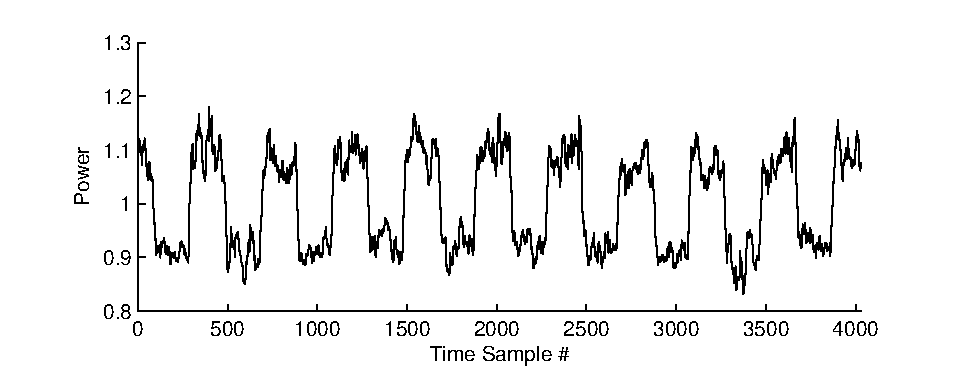
\epsfig{file=../figures/divide.eps, width=0.6\columnwidth}
%       }
% \caption{{\bf Signal Captured by the LED Light Sensor \hl{replace with a system block diagram!!}} \hl{integrates both mmm in a single design. It can operate using both RFID and TV transmissions}.}
% \label{fig:capture}
% \vskip -0.05in
% \end{figure}





\begin{figure*}[!t]
\vskip -0.1in
\centering
{\footnotesize
\begin{tabular}{ccccc}
\epsfig{file=../illustrations/waveform1.eps, width=0.4\columnwidth} & \epsfig{file=../illustrations/waveform2.eps, width=0.4\columnwidth} & \epsfig{file=../illustrations/waveform3.eps, width=0.4\columnwidth} & \epsfig{file=../illustrations/waveform4.eps, width=0.4\columnwidth} & \epsfig{file=../illustrations/waveform5.eps, width=0.4\columnwidth}\\
{(a) Normal} & {(b) Up-truncated} & {(c) Down-truncated} & {(d) Up and Down-truncated} & {(e) Average-drifted}\\
\end{tabular}
}
\vskip -0.1in
\caption{\footnotesize{\bf Varying Wave patterns.} Blah Blah.}
\label{fig:dynamicRange}
\vspace{-1em}
\end{figure*}